\titledquestion{Heap Practice}[8]
For each array provided:
\begin{enumerate}
\item Represent the array as a complete binary tree.
\item Determine if the tree is a max-heap, a min-heap, or neither.
\item If the tree is neither, convert it into a min-heap by repeatedly swapping adjacent items within the tree. Illustrate each swap by drawing the resulting sequence of trees, clearly indicating the swapped pairs on each tree.
\end{enumerate}

\begin{parts}
    \part 4, 12, 8, 21, 14, 9, 17

    \begin{solution}
        \begin{center}
            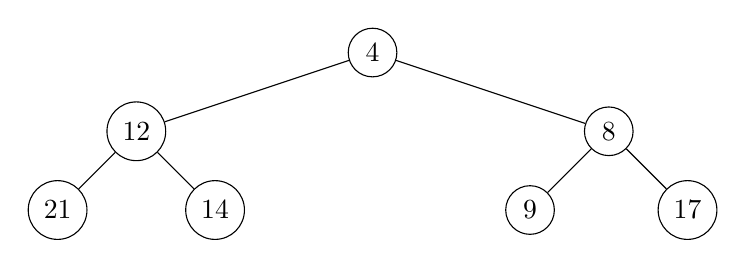
\begin{tikzpicture}[level distance=1cm,
                level 1/.style={sibling distance=2cm},
                level 2/.style={sibling distance=2cm},
                level 3/.style={sibling distance=2cm},
                every node/.style = {draw, circle}]
            \node {4}
            child {node {12}
            child {node {21}  }
            child {
                node {14}
            }
            }
            child { edge from parent[draw=none] }
            child { edge from parent[draw=none] }
            child {node {8}
            child {
                node {9}
            }
            child {
                node {17}
            }
            };
            \end{tikzpicture}
            \\
            This is a min-heap
        \end{center}
    \end{solution}

    \part 700, 250, 23, 222, 10, 21
    \begin{solution}
        \begin{center}
            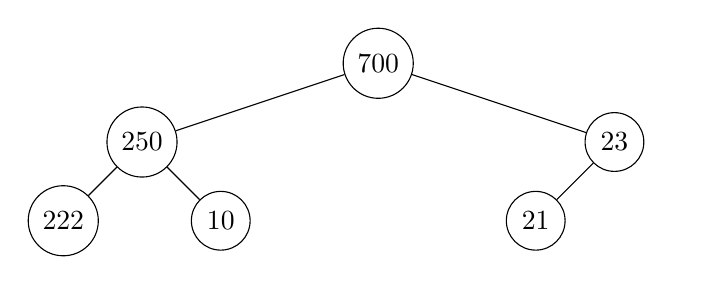
\begin{tikzpicture}[level distance=1cm,
                level 1/.style={sibling distance=2cm},
                level 2/.style={sibling distance=2cm},
                level 3/.style={sibling distance=2cm},
                every node/.style = {draw, circle}]
            \node {700}
            child {node {250}
            child {node {222}  }
            child {
                node {10}
            }
            }
            child { edge from parent[draw=none] }
            child { edge from parent[draw=none] }
            child {node {23}
            child {
                node {21}
            }
            child { edge from parent[draw=none] }
            };
            \end{tikzpicture}
            \\
            This is a max-heap
        \end{center}
    \end{solution}
    \newpage
    \part 2, 9, 13, 8, 0, 2
    \begin{solution}
        \begin{center}
            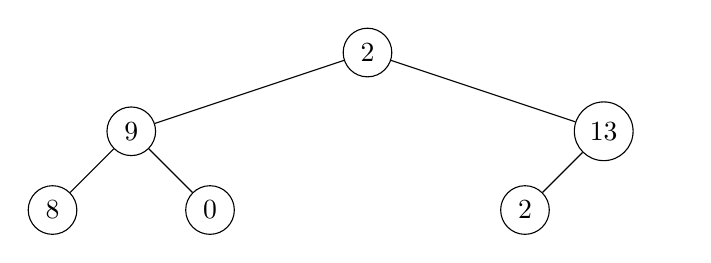
\begin{tikzpicture}[level distance=1cm,
                level 1/.style={sibling distance=2cm},
                level 2/.style={sibling distance=2cm},
                level 3/.style={sibling distance=2cm},
                every node/.style = {draw, circle}]
            \node {2}
            child {node {9}
            child {node {8}  }
            child {
                node {0}
            }
            }
            child { edge from parent[draw=none] }
            child { edge from parent[draw=none] }
            child {node {13}
            child {
                node {2}
            }
            child { edge from parent[draw=none] }
            };
            \end{tikzpicture}
            \\
            This is neither a max-heap nor a min-heap\\

            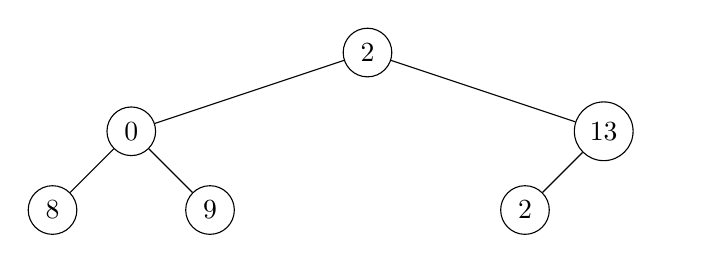
\begin{tikzpicture}[level distance=1cm,
                level 1/.style={sibling distance=2cm},
                level 2/.style={sibling distance=2cm},
                level 3/.style={sibling distance=2cm},
                every node/.style = {draw, circle}]
            \node {2}
            child {node {0}
            child {node {8}  }
            child {
                node {9}
            }
            }
            child { edge from parent[draw=none] }
            child { edge from parent[draw=none] }
            child {node {13}
            child {
                node {2}
            }
            child { edge from parent[draw=none] }
            };
            \end{tikzpicture}
            \\swap (9,0)
            \\
            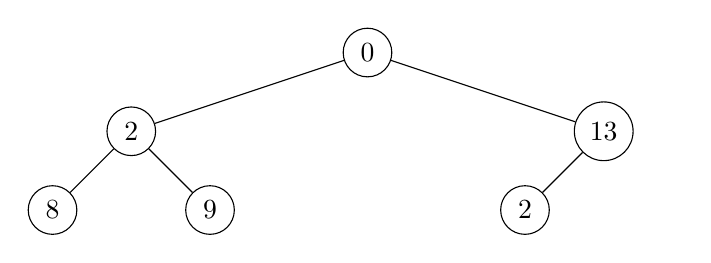
\begin{tikzpicture}[level distance=1cm,
                level 1/.style={sibling distance=2cm},
                level 2/.style={sibling distance=2cm},
                level 3/.style={sibling distance=2cm},
                every node/.style = {draw, circle}]
            \node {0}
            child {node {2}
            child {node {8}  }
            child {
                node {9}
            }
            }
            child { edge from parent[draw=none] }
            child { edge from parent[draw=none] }
            child {node {13}
            child {
                node {2}
            }
            child { edge from parent[draw=none] }
            };
            \end{tikzpicture}
            \\swap(0,2)
            \\
            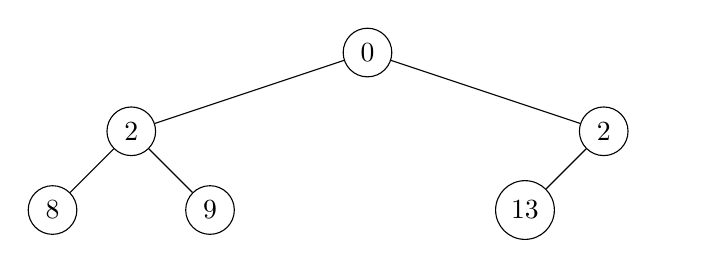
\begin{tikzpicture}[level distance=1cm,
                level 1/.style={sibling distance=2cm},
                level 2/.style={sibling distance=2cm},
                level 3/.style={sibling distance=2cm},
                every node/.style = {draw, circle}]
            \node {0}
            child {node {2}
            child {node {8}  }
            child {
                node {9}
            }
            }
            child { edge from parent[draw=none] }
            child { edge from parent[draw=none] }
            child {node {2}
            child {
                node {13}
            }
            child { edge from parent[draw=none] }
            };
            \end{tikzpicture}
            \\swap(2,13)\\
            After the swaps, the tree becomes a min-heap
        \end{center}
    \end{solution}

\end{parts}
